%%%% ijcai16.tex

\typeout{IJCAI-16 Instructions for Authors}

% These are the instructions for authors for IJCAI-16.
% They are the same as the ones for IJCAI-11 with superficical wording
%   changes only.

\documentclass{article}
% The file ijcai16.sty is the style file for IJCAI-16 (same as ijcai07.sty).
\usepackage{ijcai16}

\usepackage{tikz}
\usetikzlibrary{arrows,positioning,automata}
\usepackage[noend]{algpseudocode}
\usepackage{algorithm}
\usepackage{enumitem, kantlipsum}

% Use the postscript times font!
\usepackage{times}

\usepackage{mathtools}
\usepackage{amssymb}

\DeclareMathAlphabet{\mathrmbf}{\encodingdefault}{\rmdefault}{bx}{n}
% the following package is optional:
%\usepackage{latexsym} 

% Following comment is from ijcai97-submit.tex:
% The preparation of these files was supported by Schlumberger Palo Alto
% Research, AT\&T Bell Laboratories, and Morgan Kaufmann Publishers.
% Shirley Jowell, of Morgan Kaufmann Publishers, and Peter F.
% Patel-Schneider, of AT\&T Bell Laboratories collaborated on their
% preparation.

% These instructions can be modified and used in other conferences as long
% as credit to the authors and supporting agencies is retained, this notice
% is not changed, and further modification or reuse is not restricted.
% Neither Shirley Jowell nor Peter F. Patel-Schneider can be listed as
% contacts for providing assistance without their prior permission.

% To use for other conferences, change references to files and the
% conference appropriate and use other authors, contacts, publishers, and
% organizations.
% Also change the deadline and address for returning papers and the length and
% page charge instructions.
% Put where the files are available in the appropriate places.
% \thanks{These match the formatting instructions of IJCAI-07. The support of
% IJCAI, Inc. is acknowledged.}

\title{Appraisal Algorithms for Relevance and Controllability in\\
Human-Robot Collaboration}
% \author{Mahni Shayganfar, Charles Rich, Candace L. Sidner \\ 
% Worcester Polytechnic Institute, Worcester Massachusetts  \\
% mshayganfar $|$ rich $|$ sidner @wpi.edu}

\begin{document}

\maketitle

\begin{abstract}
\vspace*{-1mm}
We have investigated the mutual influences of affective and collaborative
processes in a cognitive theory to support interaction between humans and robots
or virtual agents. We build primarily on the \textit{cognitive appraisal} theory of
emotions and the \textit{SharedPlans} theory of collaboration to investigate the
structure, fundamental processes and functions of emotions in a collaboration.
We have developed new algorithms for appraisal processes as part of a new
overall computational model. We have evaluated our implemented algorithms by
conducting an online user study.
\end{abstract}

\vspace*{-3mm}
\section{Introduction}
% Sousa in The Rationality of Emotion \cite{sousa:rationality-emotion}
% makes the case for claiming that humans are capable of rationality largely
% because they are creatures with emotions. 
The idea of robots or other intelligent agents living in a human environment has
been a persistent dream from science fiction books to artificial intelligence
and robotic laboratories. Collaborative robots are expected to become an
integral part of humans' environment to accomplish their industrial and
household tasks. In these environments, humans will be involved in robots'
operations and decision-making processes. The involvement of humans influences
the efficiency of robots' interaction and performance, and makes the robots
sensitive to humans' cognitive abilities and behaviors.

This work is implemented as part of a larger effort to build robots capable of
generating and recognizing emotions in order to be better collaborators. In this
paper, we report on the specific problem of appraising the relevance and
controllability of events within a collaborative interaction. Our contribution
is to ground general appraisal concepts in the specific context and structure of
collaboration. This work is part of the development of \textit{Affective
Motivational Collaboration Theory} which is built on the foundations of the
\textit{SharedPlans} theory of collaboration \cite{grosz:plans-discourse} and
the \textit{cognitive appraisal} theory of emotions
\cite{gratch:domain-independent}.

There are several appraisal models (e.g., EMA \cite{marsella:ema-process-model})
contributing in different applications such as social sciences, virtual agents,
and robotics. However, none of these models have focused on the appraisal
processes during collaboration. We believe appraisal plays a key role in
collaboration due to its regulatory and evaluative nature. Also, collaboration
induces some changes to underlying appraisal processes due to its unique nature.
For instance, although the appraisal models mostly use utility to compute the
relevance of an event, we have found new cognitive components involved in
determining utility because of the influence of the collaboration. These
components, such as the recurrence of a belief by the human collaborator or the
influence of the human collaborator's perceived emotion on the robot's decisions
emphasize the fact that collaboration requires different procedures in appraisal
processes. In this paper, we provide the relevance and controllability
appraisals of an event in the collaboration context.

% After discussing related works, we briefly introduce the Affective Motivational
% Collaboration Theory, focusing on the collaboration and appraisal mechanisms as
% well as mental states. We then provide more details about the graph
% representation of the robot's mental state. Next, we describe the algorithms we
% developed to compute the value of four crucial appraisal variables. To compare
% the results from our algorithms with humans' decisions we have conducted a user
% study using crowd sourcing; the results are provided in Section
% \ref{sec:user-study}.

\vspace*{-2mm}
\section{Related Work}
\vspace*{-1mm}
Our work builds on the general notions of appraisal theory
\cite{gratch:domain-independent,marsella:computational,scherer:sequential-appraisal-process,scherer:appraisal-processes},
but is focused on its application in human-robot collaboration. Computational
appraisal models have been applied to a variety of uses in psychology, robotics,
AI, and cognitive science. For instance, in \cite{marsella:ema-process-model}
EMA is used to generate specific predictions about how human subjects will
appraise and cope with emotional situations. Furthermore, appraisal theory has
been used in robots' decision making \cite{castro:autonomous-robot-fear}, or in
their cognitive systems
\cite{hudlicka:emotinos-reasons,marinier:emotion-reinforcement}. In the virtual
agents community, empathy and affective decision-making is a research topic that
has received much attention in the last two decades
\cite{scott:modeling-empathy-agent,paiva:agent-care,pontier:women-robot-men,velasquez:emotions-motivations-agents}.
However, EMA and other work in artificial intelligence and robotics which apply
appraisal theory do not focus on the dynamics of collaborative contexts
\cite{adam:bdi-emotional-companion,kim:model-hri-appraisal,marsella:ema-process-model,rosenbloom:sigma-appraisal}.

The computational collaboration model in our work is strongly influenced by the
SharedPlans theory \cite{grosz:plans-discourse}. However, our algorithms are
also compatible with other collaboration theories, e.g., Joint Intentions theory
\cite{cohen:teamwork}, or STEAM \cite{tambe:flexible-teamwork}. These theories
have been extensively used to examine and describe teamwork and collaboration.
Yet, collaboration and emotion theories have never been combined, as they are in
our work. We believe a systematic integration of collaboration theories and
appraisal theory can help explain the underlying processes OF collaboration
structure.

\section{{\fontsize{11.85}{12}\selectfont Affective Motivational Collaboration
Theory}}

Affective Motivational Collaboration Theory deals with the interpretation and
prediction of observable behaviors in a dyadic collaboration
\cite{shayganfar:appraisal-short}. The theory focuses on the processes regulated
by emotional states. The observable behaviors represent the outcome of reactive
and deliberative processes related to the interpretation of the self's
relationship to the environment. Affective Motivational Collaboration Theory
aims to explain both rapid emotional reactions to events as well as slower, more
deliberative responses. The reactive and deliberative processes are triggered by
two types of events: \textit{external} events, such as the other's
\textit{utterances} and \textit{primitive actions}, and \textit{internal}
events, comprising changes in the self's mental states, such as belief formation
and emotional changes. The theory explains how emotions regulate the underlying
processes when these events occur. It also elucidates the role of
\textit{motives} as goal-driven emotion-regulated constructs with which a robot
can form new intentions to cope with events.

\vspace*{-3mm}
\begin{figure}[tbh]
  \centering
  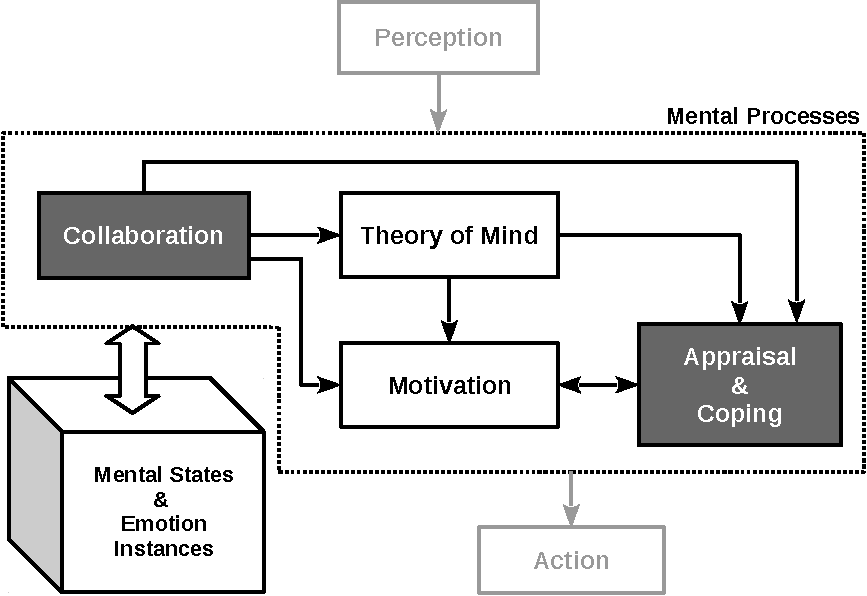
\includegraphics[width=0.45\textwidth]{figure/theory-general-croped.pdf}
  \vspace*{-3mm}
  \caption{{\fontsize{9}{9}\selectfont Computational framework based on
  Affective Motivational Collaboration Theory (arrows indicate primary
  influences between mechanisms).}}
  \vspace*{-3mm}
  \label{fig:cpm}
\end{figure}

Our focus is on the mechanisms depicted as mental processes in Figure
\ref{fig:cpm} along with the mental states. Each mechanism includes one or
more processes in our architecture. For instance, the \textit{Collaboration}
mechanism includes processes such as \textit{Focus Shifting} and
\textit{Constraint Management}, while as we discuss in Section
\ref{sec:appraisal-process} the \textit{Appraisal} mechanism includes processes
to compute the values for different appraisal variables. The \textit{mental
states} includes self's (robot's) beliefs, intentions, motives, goals and
emotion instances as well as the anticipated mental states of the other (human).
The \textit{Collaboration} mechanism maintains constraints on actions, including
task states and the ordering of tasks, and provides processes to update and
monitor the shared plan. The \textit{Appraisal} mechanism is responsible for
evaluating changes in the self's mental states, the anticipated mental states of
the other, and the state of the collaboration environment. The \textit{Coping}
mechanism provides the self with different coping strategies associated with
changes in the self's mental states with respect to the state of the
collaboration. The \textit{Motivation} mechanism operates whenever the self a)
requires a new motive to overcome an internal impasse in an ongoing task, or b)
wants to provide an external motive to the other when the other faces a problem
in a task. The \textit{Theory of Mind} mechanism infers a model of the other's
anticipated mental state. The self progressively updates this model during the
collaboration.

\vspace*{-2mm}
\subsection{Mental States}
\label{sec:mental-states}
\vspace*{-2mm}
A brief description of mental states is provided as prerequisite knowledge for
understanding the appraisal processes. The mental states shown in Figure
\ref{fig:cpm} comprise the knowledge base required for all the mechanisms in the
overall model. Mental states are conscious states of mind providing the content
for cognitive processes. These mental states possess attributes, each of which
provides a unique interpretation of the related cognitive entities. The self
uses these attributes whenever there is an arbitration in the internal cognitive
processes. We only describe some of the attributes of beliefs and motives in
this paper, since they are used in our appraisal algorithms.

\textit{Beliefs} are a crucial part of the mental states. Beliefs have
attributes and they impact different processes of the framework such as the
evaluation of an external event by the Appraisal mechanism, and updates to the
collaboration plan. We use three belief attributes in the Appraisal mechanism.
Belief \textit{strength} is about how strongly the self holds salient beliefs
about an object, an entity, or an anticipated behavior. The \textit{saliency} of
a belief is a cognitive attribute that pertains to how easily the self becomes
aware of a belief. The \textit{persistence} of a belief refers to how resistant
the belief is to changes.

\textit{Motives} are mental constructs which can initiate, direct and maintain
goal-directed behaviors. They are created by the emotion-regulated Motivation
mechanism. Motives can cause the formation of a new intention for the robot
according to: a) its own emotional states, b) its own private goal, c) the
collaboration (shared) goal, and d) other's anticipated beliefs. Motives possess
a set of attributes. The Motivation mechanism compares motives based on the
quality of these attributes and chooses the one which is the most related to the
current state of the collaboration. We use two motive attributes in Appraisal
mechanisms. The \textit{importance} of a motive is determined by the
corresponding beliefs about the effects of achieving or not achieving the
associated goal. The \textit{urgency} of a motive defines how much time the self
has to acknowledge and address that motive before it is too late.

\textit{Intentions} are mental constructs directed at goals and future actions.
They play an essential role in taking actions according to the collaboration
plan as well as behavior selection in the Coping mechanism. Intentions are
also involved in selecting intention-related strategies, e.g., planning, seeking
instrumental support and procrastination. 

% Intentions possess a set of
% attributes, i.e., \textit{Temporal Status, Direct Experience, Certainty,
% Ambivalence, Affective-Deliberative Consistency} which moderate the consistency
% between intention and behavior \cite{cooke:intention-behavior-consistency}. The
% details about these attributes are beyond the scope of this paper.

\textit{Goals} help the robot to create and update its collaboration plan
according to the current private and shared goal content and structure. Goals
direct the formation of intentions to take appropriate corresponding actions
during collaboration. 

% Goals also drive the Motivation mechanism to generate
% required motive(s). The details about goal's attributes are beyond the scope of
% this paper.

\textit{Emotions} in mental states are emotion instances that are elicited by
the Appraisal mechanism, e.g., \textit{Joy, Anger, Hope, Worry}. These emotion
instances include the robot's own emotions as well as the anticipated emotions
of the other which are created with the help of the processes in the Theory of
Mind mechanism. 

% Each emotion has its own functionality in either the
% intrapersonal or interpersonal level. These emotions not only regulate the
% self's internal processes, but also assist the self to anticipate the other's
% mental states.

\begin{figure*}
  \centering
  \vspace*{-5mm}
  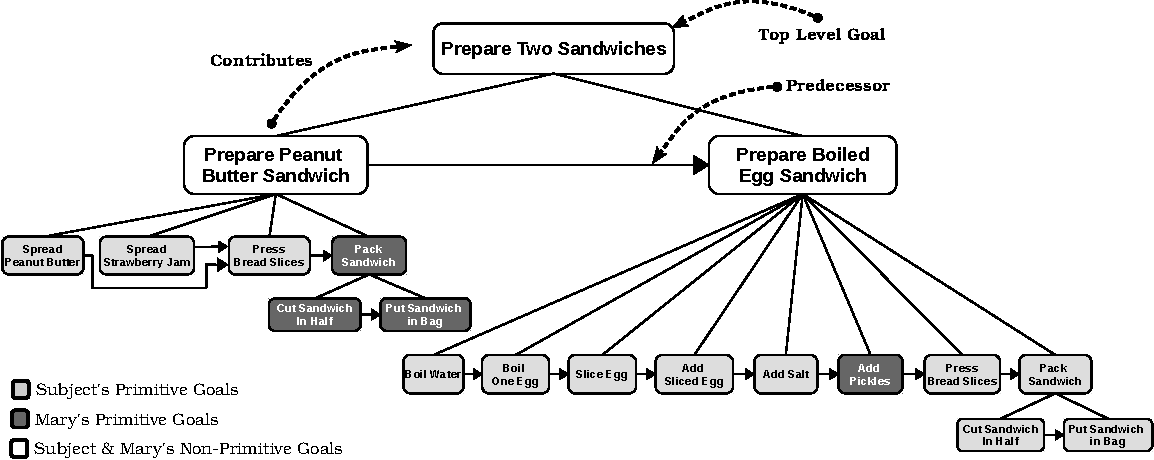
\includegraphics[width=14.5cm,height=5cm]{figure/taskModel-croped.pdf}
  \vspace*{-3mm}
  \caption{Example of collaboration structure (also used as task model for
  the evaluation).}
  \label{fig:taskModel}
  \vspace*{-4mm}
\end{figure*}

% \section{Example Scenario}
% 
% The example scenario is part of a much larger interaction we are implementing to
% test our theory. This example shows a very short part of an interaction between
% a robot and an astronaut during their collaboration. Their mission is to finish
% installing a few solar panels together. However, the astronaut encounters a
% measurement tool problem:
% 
% \begin{description}
%   \item \textit{\textbf{\fontsize{9pt}{12pt}\selectfont Astronaut [turn t-1]:}}
%   Oh no! Finishing the quality check of our installation with this measurement
%   problem is so frustrating. I think we should stop now!
% 
%   \item \textit{\textbf{\fontsize{9pt}{12pt}\selectfont{Robot [turn t]:}}}
%   I see. This is frustrating. But, I can help you with the measurement tool and
%   we can finish the task as originally planned.
% \end{description}
% 
% \vspace*{-1mm}
% In this scenario, the robot appraises the problem with the measurement tool as
% a \textit{relevant, undesirable, unexpected}, but \textit{controllable} event.
% Consequently, the coping mechanism first acknowledges the astronaut's negative
% valenced emotion (i.e., frustration), then provides a new plan to continue the
% collaboration.

\vspace*{-3mm}
\section{Collaboration}
\label{sec:collaboration}

The Collaboration mechanism constructs a hierarchy of goals associated with
tasks in a hierarchical task network (see Figure \ref{fig:taskModel}), and also
maintains the constraints and other required details of the collaboration
including the inputs and outputs of individual tasks, the \textit{preconditions}
(specifying whether it is appropriate to perform a task), and the
\textit{postconditions} (specifying whether a just-completed task was
successful). Collaboration also monitors the focus of attention, which
determines the salient objects, properties and relations at each point, and
shifts the focus of attention during the interaction.

% \vspace*{-2mm}
% \begin{figure}[tbh]
%   \centering
%   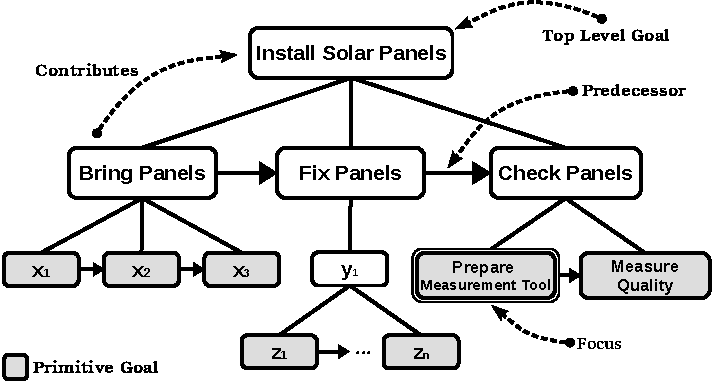
\includegraphics[width=0.474\textwidth]{figure/collaborationStructure-croped.pdf}
%   \vspace*{-4mm}
%   \caption{{\fontsize{9}{9}\selectfont Collaboration structure (shared plan).}}
%   \label{fig:cs}
%   \vspace*{-2mm}
% \end{figure}

Here, we describe the methods which retrieve information about the collaboration
structure, and are used to compute the values of appraisal variables. In these
methods, $\varepsilon_t$ is the event corresponding to time \textit{t}, and
$g_t$ is a given goal at time \textit{t}.

\begin{itemize}[leftmargin=2pt]
  \setlength\itemsep{0.02mm}
  \item \textit{recognizeGoal($\varepsilon_t$)} returns the unique goal to which
  the given event (action, utterance, or emotional expression) directly
  contributes; it is only one goal since the robot can only do one primitive
  action at a time in our collaboration model, i.e, in the goal tree, a given
  primitive action can only directly contribute to one parent goal. The method
  returns \textit{ambiguous} if it does not recognize a goal in the
  plan\footnote{Ambiguity introduces some extra complexities which are beyond
  scope of this paper.}.
   
%   \item \textit{topLevelGoalStatus($g_t$)} returns the status of the top level
%   goal whether it is \textsc{achieved, failed, blocked, inapplicable, pending,}
%   or \textsc{in progress}. In our example, ``Prepare Two Sandwiches'' is the top
%   level goal.
  
  \item \textit{getGoalStatus($g_t$)} returns whether $g_t$'s status is
  \textsc{achieved, failed, blocked, inapplicable, pending,} or \textsc{in
  progress}. In our example, ``Add Pickles'' is the current (focused) goal and
  it is \textsc{pending}, and the ``Prepare Boiled Egg Sandwich'' and ``Prepare
  Two Sandwiches'' are in \textsc{in progress}. The focused goal is the goal
  that the robot currently pursues.
  
  \item \textit{precondStatus($g_t$)} returns the status of the $g_t$'s
  precondition, i.e., whether it is \textsc{satisfied, unsatisfied} or
  \textsc{unknown}. For instance, the precondition for ``Slice Egg'' can
  indicate whether the eggs are boiled appropriately, i.e., \textsc{satisfied}.
  
  \item \textit{isLive($g_t$)} returns \textit{true} if all the predecessors of
  $g_t$ are \textsc{achieved} and all the preconditions are \textsc{satisfied},
  i.e., \textsc{pending} or \textsc{in progress} goals; otherwise returns \textit{false}.
  
%   \item \textit{isFocusShift($g_t$)} returns \textit{true} if the given
%   goal is not the previous focus (top of the stack); otherwise returns
%   \textit{false}.
  
%   \item \textit{isNecessaryFocusShift($g_t$)} returns \textit{true} if the
%   status of the previous focus was \textsc{achieved}; otherwise returns
%   \textit{false} \cite{rich:focused-unfocused-users}.
  
%   \item \textit{isPath($g_1$, $g_2$)} returns \textit{true} if there is a path
%   between $g_1$ and $g_2$ in a plan tree structure; otherwise returns
%   \textit{false}.
  
%   \item \textit{doesContribute($g_t$)} returns whether the given goal
%   contributes to another goal in the higher level of the plan hierarchy. For
%   instance, an abstract (nonprimitive) goal of ``Prepare Peanut Butter
%   Sandwich'' contributes to the higher level goal of ``Prepare Two Sandwiches''.
  
  \item \textit{getContributingGoals($g_t$)} returns $g_t$'s children.
    
  \item \textit{getPredecessors($g_t$)} returns $g_t$'s predecessors.
  
  \item \textit{getInputs($g_t$)} returns all required inputs for $g_t$. For
  example, the goal ``Boil Water'' requires inputs such as \textit{Pot} and
  \textit{Stove} (details not shown in Figure \ref{fig:taskModel}).
  
  \item \textit{isAvailable($g_t, i_{_k}$)} returns whether the given input
  ($i_{_k}$) is available for $g_t$. For instance, whether the \textit{Pot} is
  available for the goal ``Boil Water''.
  
%   \item \textit{isAchieved($g_t$)} returns whether the given goal is achieved,
%   i.e., whether all the postconditions of the given goal are \textsc{satisfied}.
  
  \item \textit{isFocused($g_t$)} returns whether the focus is on $g_t$.
  
  \item \textit{getResponsible($g_t$)} returns responsible agent(s) for $g_t$.
  In a dyadic collaboration, both of the agents (joint) can be partly responsible
  for a nonprimitive goal, while each (self or other) is responsible for one or
  more primitive goals. For instance, both Mary and the subject are responsible
  for the nonprimitive goal ``Prepare Boiled Egg Sandwich'', whereas only Mary
  is responsible for the primitive goal ``Add Pickles''.
\end{itemize}

\vspace*{-5mm}
\section{Appraisal Processes}
\label{sec:appraisal-process}

We discuss two appraisal variables in a collaboration context, i.e.,
\textit{relevance} (since other appraisals are only computed for relevant
events), and \textit{controllability} (since it is associated with the agent's
coping ability). There are other appraisal variables introduced in psychological
\cite{scherer:appraisal-processes} and computational literature
\cite{gratch:domain-independent}. We have implemented other appraisal variables
such as \textit{expectedness} \cite{shayganfar:appraisal-short} and
\textit{desirability} \cite{shayganfar:emotional-awareness} which do not appear
in this paper due to space limitations. The algorithms in this section use
mental states of the robot (see Section \ref{sec:mental-states}) which are
formed based on the collaboration structure.

\vspace*{-2mm}
\subsection{Relevance}

Relevance as an appraisal variable measures the significance of an event for the
self. An event can be evaluated to be relevant if it has a non-zero utility
\cite{marsella:ema-process-model}. Relevance is an important appraisal variable
since the other appraisal variables are meaningful only for relevant events.
However, the utility of an event during collaboration is influenced by the other
collaborator's actions and mental states, because there is a commitment between
collaborators to achieve the shared goal based on the shared plan. Other
appraisal models only consider the utility of an event based on the self's
(robot's) goal and plan.

Algorithm \ref{alg:relevance} determines the relevance of the given event with
respect to the current mental state. The relevance of the event depends on the
significance of the event with respect to the collaboration status, which is
determined based on the utility of the event as presented in
\cite{gratch:domain-independent,marsella:ema-process-model}. Our algorithm for
computing the relevance of an event during collaboration involves other factors
that other appraisal models do not consider. For instance, the human's
perceived emotion, recurrence of a belief, or occurrence of a belief about an
unrelated goal by the human play important roles by influencing the utility
of an event during collaboration. As a result, evaluating the relevance of
events can cause a collaborative robot to respond effectively which can
positively impact the status of the shared goal, without dedicating all its
resources to every event.

\vspace*{-3mm}
\begin{algorithm}
	\caption{(Relevance)}
	\label{alg:relevance}
	\begin{algorithmic}[1]
		\Function{IsEventRelevant}{Event $\varepsilon_t$}
% 			\Statex
			\State $\mathit{g}_{t} \gets \textit{recognizeGoal}{(\varepsilon_t)}$
% 			\Statex
			\State $\mathcal{U} \gets \Call{getEventUtility}{\mathit{g}_{t}}$ 
			\State $\tau_{t} \gets \Call{getEmotionalThreshold}{\mathit{g}_{t}}$
% 			\Statex
			\If {$(\tau_{t} \leq |\mathcal{U}|)$} \quad \Return
			{{\fontsize{7}{8}\selectfont RELEVANT}} 
% 				\State \Return {{\fontsize{7}{8}\selectfont RELEVANT}}
			\Else \quad \Return {{\fontsize{7}{8}\selectfont IRRELEVANT}}
% 				\State \Return {{\fontsize{7}{8}\selectfont IRRELEVANT}}
			\EndIf
		\EndFunction
	\end{algorithmic}
\end{algorithm}

\vspace*{-3mm}
After perceiving an event, the belief about that event represents the event in
the robot's mental state. \textit{recognizeGoal} returns the goal to which the
current event contributes. We compute the utility ($-1 \leq \mathcal{U} \leq 1$)
of the event using the values of the attributes associated with the existing
beliefs, and the attributes of the motive associated with the recognized goal
(see details below). We use three belief attributes (see Section
\ref{sec:mental-states}) to compute the belief-related part of the utility:

\vspace*{-1mm}
\begin{itemize}[leftmargin=2pt]
  \setlength\itemsep{0.025mm}
  \item \textit{Strength (T)}: The extent to which the preconditions ($\alpha$),
  postconditions ($\beta$), predecessors ($\lambda$), and contributing goals
  ($\mu$) of a goal are known (\textsc{satisfied} or \textsc{unsatisfied}) makes
  beliefs about the goal stronger. An \textsc{unknown} pre/postcondition status
  of a goal and its predecessors and contributing goals forms weaker beliefs.
  For instance, if one knows all predecessors of a pursued goal (e.g., ``Press
  Bread Slices'') are \textsc{satisfied} (i.e., ``Spread Peanut Butter'' and
  ``Spread Strawberry Jam''), failure of the pursued goal will elicit one's
  negative emotion (due to the strong beliefs related to the goal); whereas not
  knowing the status of the goal-related factors (e.g., whether Mary could find
  the knife to cut the sandwich in half) causes one to form weaker beliefs about
  the goal.
  \item \textit{Saliency (S)}: Beliefs related to the focused goal are more
  salient than beliefs related to any other goal in the plan. For example,
  according to Figure \ref{fig:taskModel}, if one is making a boiled egg
  sandwich, beliefs related to all of the \textit{live} (\textsc{pending} or
  \textsc{in progress}) goals (e.g. ``Pack Sandwich'') will be less salient
  than beliefs related to the focused goal, i.e., ``Add Pickles''. Beliefs'
  saliency decreases according to their corresponding \textit{live} goal's
  distance from the focused goal in the shared plan. \textit{Non-live} goals
  will not be salient.
  \item \textit{Persistence (P)}: The recurrence of a belief over time (turns)
  increases the persistence of the belief. Beliefs occurring only once have the
  lowest value of persistence. For instance, if Mary keeps saying that she can
  not find the knife to cut the sandwich in half, one could pursue a new goal
  outside of the shared plan to acknowledge Mary's concern.
\end{itemize}

\noindent We also use two motive attributes discussed in Section
\ref{sec:mental-states} to compute the motive related part of the utility
($\mathcal{U}$):

\begin{itemize}[leftmargin=2pt]
  \setlength\itemsep{0.05mm}
  \item \textit{Urgency ($\gamma$)}: There are two factors impacting the urgency
  of a motive: a) whether the goal directing the given motive is the predecessor of
  another goal for which the other collaborator is responsible, and b) whether
  achieving the goal directing the given motive can mitigate the other
  collaborator's negative valenced emotion. For instance, if one has a private
  goal to prepare for making the second sandwich (e.g. get the eggs) while Mary
  is waiting to get the first sandwich and cut it in half, pressing bread slices
  and passing them to Mary will be more urgent than one's private goal.
  \item \textit{Importance ($\eta$)}: A motive is important if failure of the
  directing goal causes an impasse in the shared plan (i.e., no further goal is
  available to achieve), or achievement of the directing goal removes an
  existing impasse. For example, if one cannot find white bread on which to
  spread peanut butter (an impasse to make the peanut butter sandwich), and Mary
  offers to use wheat bread instead (external motive), the new motive becomes
  important to remove the impasse in the shared plan.
\end{itemize}

We provide the utility function in Equation \ref{eqn:utility}. This function is
comprised of: a) saliency (\textit{S}) and b) persistence (\textit{P}) of the
belief(s) related to the recognized goal, c) the recognized goal's status
($\upsilon$), and d) aggregation of belief and motive attributes ($\Psi$) using
the function in Equation \ref{eqn:power}.

\vspace*{-3mm}
\begin{equation}
    U(\varepsilon_t)= 
    \begin{dcases}
       \upsilon\!P\cdot S^{\Psi} & \Psi \textgreater 0 \\
       0               			 & \Psi = 0
    \end{dcases}
    \label{eqn:utility}
\end{equation}

In equation \ref{eqn:power}, the subscript \textit{k} refers to the
\textit{known} goal-related factors (\textsc{satisfied} or
\textsc{unsatisfied}); whereas the subscript \textit{all} includes both
\textit{known} and \textit{unknown} goal-related factors. In this equation, both
urgency ($\gamma$) and importance ($\eta$) attributes of motives can impact the
outcome of the goal-related belief attributes' ratio, and ultimately the $\Psi$
value.

\vspace*{-3mm}
\begin{equation}
    \Psi = \frac{\alpha_{_k} + \beta_{_k} + \lambda_{_k} +
    \mu_{_k}}{\alpha_{_{all}} + \beta_{_{all}} + \lambda_{_{all}} +
    \mu_{_{all}}} + \eta + \gamma
    \label{eqn:power}
\end{equation}

\vspace*{-1mm}
\begin{center} 
    $\eta, \gamma \in \mathbb{N}, \qquad\qquad \eta, \gamma \geq 0$\\
    $\alpha_{_k}, \beta_{_k}, \lambda_{_k}, \mu_{_k} \in \mathbb{N},
    \qquad\qquad \alpha_{_k}, \beta_{_k}, \lambda_{_k}, \mu_{_k} \geq 0$\\
    $\alpha_{_{all}}, \lambda_{_{all}}, \mu_{_{all}} \in \mathbb{N},
    \qquad\qquad \alpha_{_{all}}, \lambda_{_{all}}, \mu_{_{all}} \geq 0$\\
    $\beta_{_{all}} \in \mathbb{N}, \qquad\qquad \beta_{_{all}} \geq 1$
\end{center}

Intuitively, $\Psi$ value indicates the quality of beliefs and motives using
their attributes. Hence, the $\Psi$ value impacts the saliency value of
beliefs exponentially helping to differentiate between beliefs. Similarly,
\textit{P} influences the value of utility only as a coefficient since recurrent
beliefs are not formed frequently during collaboration. We use $\upsilon$ to
generate positive and negative utility values. The $\upsilon$'s value becomes +1
if the status of the corresponding goal is \textsc{achieved}, \textsc{pending},
or \textsc{in progress}, and $\upsilon$'s value becomes -1 if the status of the
corresponding goal is \textsc{failed, blocked, inapplicable}.

The significance of an event in a collaborative environment is based on the
utility of the event and the perceived emotion of the human collaborator. The
human's emotion influences the relevance the event in the form of a threshold
value $\tau_{t}$ (see Algorithm \ref{alg:relevance}). For instance, a positively
expressed emotion of the human reduces the threshold value which makes the robot
find an event relevant with even a slightly positive utility. This threshold
value is currently determined based on whether the valence of the human's
perceived emotion is positive (e.g., happiness) or negative (e.g., anger).
Therefore, an event can be considered \textsc{irrelevant} even though the
utility has a relatively positive value, because relevance is influenced by the
human's perceived negative emotion.

% \vspace*{-1mm}
% \subsection{Desirability}
% 
% Desirability characterizes the value of an event to the robot in terms of
% whether the event facilitates or thwarts the collaboration goal. Desirability
% captures the valence of an event with respect to the robot's preferences
% \cite{gratch:domain-independent}. In a collaborative robot, preferences are
% biased towards those events facilitating progress in the collaboration.
% Desirability plays an important role in the overall architecture; it makes the
% processes involved in the other mechanisms (e.g., Motivation and Theory of
% Mind), and consequently the robot's mental state, congruent with the
% collaboration status which is a collaborative robot's desire. Therefore, it
% causes the robot to dismiss events causing inconsistencies in the robot's
% collaborative behavior. Moreover, desirability is also crucial from the
% collaboration's point of view.
% 
% Algorithm \ref{alg:desirability} provides a process in which the desirability of
% an event is computed with regard to the status of the shared goal; i.e., it
% operates based on whether and how the event changes the status of the current
% shared goal. It distinguishes between the top level goal and the current goal
% because the top level goal's change of status attains a higher positive or
% negative value of desirability. For instance, failure of the top level goal
% (e.g., installing solar panel) is more undesirable than failure of a primitive
% goal (e.g., measuring the quality of the installed panel).
% 
% An \textsc{ambiguous} goal is a goal associated with the current event
% ($\varepsilon_t$) which is not recognized in the robot's plan; therefore it is
% \textsc{undesirable} for a collaborative robot. A top level goal' status must be
% \textsc{achieved} (i.e., \textsc{satisfied} postcondition) to consider the event
% \textsc{most-desirable}. When the goal's status is \textsc{failed} (i.e.,
% \textsc{unsatisfied} postcondition) or \textsc{blocked}, the associated event
% has the \textsc{most-undesirable} or \textsc{undesirable} values respectively.
% A goal is \textsc{blocked} if any of the required goals or goals recursively
% through the parent goal are not \textsc{achieved}. An \textsc{inapplicable} goal
% is also considered as \textsc{undesirable}. A goal is \textsc{inapplicable} if
% any of its predecessors are not \textsc{achieved}, and/or its preconditions are
% not \textsc{satisfied}. For \textsc{pending} and \textsc{inprogress} top level
% goals, the status of the current goal associated with the top level goal
% determines the status of the event $\varepsilon_t$. Only a non-primitive goal
% can have \textsc{inprogress} status, if it has been started but is not yet
% completed. A goal can be \textsc{pending} if it is live, or if it is a
% non-primitive goal that has not been started yet. \textsc{Achieved} current
% goals mark an event ($\varepsilon_t$) as \textsc{desirable}, while
% \textsc{failed} or \textsc{blocked} current goals render the event associated
% with them as \textsc{most-undesirable} and \textsc{undesirable} respectively.
% \textsc{Pending} or \textsc{inprogress} current goals mark their associated
% events as \textsc{neutral}.
% 
% \vspace*{-1mm}
% \begin{algorithm}
% 	\caption{(Desirability)}
% 	\label{alg:desirability}
% 	\begin{algorithmic}[1]
% 		\Function{IsEventDesirable}{Event $\varepsilon_t$}
% % 			\Statex
% 			\State $\mathit{g}_{t} \gets \textit{recognizeGoal}{(\varepsilon_t)}$
% % 			\Statex
% 			\If {$(\mathit{g}_{t} =$ {\fontsize{7}{8}\selectfont AMBIGUOUS}$)$} 
% 				\State \Return {\fontsize{7}{8}\selectfont UNDESIRABLE}
% 			\EndIf
% % 			\Statex
% 			\If {{\fontsize{8}{9}\selectfont(\textit{topLevelGoalStatus($g_{t}$)} =
% 			{\fontsize{7}{8}\selectfont ACHIEVED})}} 
% 			\State \Return {{\fontsize{7}{8}\selectfont MOST-DESIRABLE}} 
% 			\ElsIf {{\fontsize{8}{9}\selectfont(\textit{topLevelGoalStatus($g_{t}$)}} =
% 			{\fontsize{7}{8}\selectfont FAILED})} 
% 			\State \Return {{\fontsize{7}{8}\selectfont MOST-UNDESIRABLE}}
% 			\ElsIf {{\fontsize{8}{9}\selectfont(\textit{topLevelGoalStatus($g_{t}$)}} =
% 			{\fontsize{7}{8}\selectfont BLOCKED}) \OR\\
% 			\hspace{1mm}{\fontsize{8}{9}\selectfont
% 			\hspace*{4mm}(\textit{topLevelGoalStatus($g_{t}$)}} =
% 			{\fontsize{7}{8}\selectfont INAPPLICABLE)}} 
% 			\State \Return {{\fontsize{7}{8}\selectfont UNDESIRABLE}} 
% 			\ElsIf {{\fontsize{8}{9}\selectfont(\textit{topLevelGoalStatus($g_{t}$)}} =
% 			{\fontsize{7}{8}\selectfont PENDING}) \OR\\
% 			\hspace{1mm}{\fontsize{8}{9}\selectfont
% 			\hspace*{4mm}(\textit{topLevelGoalStatus($g_{t}$)}} =
% 			{\fontsize{7}{8}\selectfont INPROGRESS})}
% % 				\Statex
% 				\If {{\fontsize{8}{9}\selectfont (\textit{currGoalStatus($g_{t}$)}} =
% 				{\fontsize{7}{8}\selectfont ACHIEVED})}
% 				\State \Return {{\fontsize{7}{8}\selectfont DESIRABLE}}
% 				\ElsIf {(\textit{currGoalStatus($g_{t}$)} = {\fontsize{7}{8}\selectfont
% 				FAILED})} 
% 				\State \Return {{\fontsize{7}{8}\selectfont MOST-UNDESIRABLE}}
% 				\ElsIf {(\textit{currGoalStatus($g_{t}$)} = {\fontsize{7}{8}\selectfont
% 				BLOCKED}) \OR \\
% 				\hspace{1mm}{\fontsize{8}{9}\selectfont
% 				\hspace*{9mm}(\textit{topLevelGoalStatus($g_{t}$)}} =
% 				{\fontsize{7}{8}\selectfont INAPPLICABLE})} 
% 				\State \Return {{\fontsize{7}{8}\selectfont UNDESIRABLE}}
% 				\ElsIf {{\fontsize{8}{9}\selectfont(\textit{topLevelGoalStatus($g_{t}$)}} =
% 				{\fontsize{7}{8}\selectfont PENDING}) \OR \\ \hspace{1mm} 
% 				\hspace*{8mm}(\textit{currGoalStatus($g_{t}$)} =
% 				{\fontsize{7}{8}\selectfont INPROGRESS})} 
% 				\State \Return {{\fontsize{7}{8}\selectfont NEUTRAL}}
% 				\EndIf
% 			\EndIf
% 		\EndFunction
% 	\end{algorithmic}
% \end{algorithm}
% 
% \vspace*{-1mm}
% \subsection{Expectedness}
% 
% Expectedness is the extent to which the truth value of a state could have been
% predicted from causal interpretation of an event
% \cite{marsella:ema-process-model}. In the collaboration context the expectedness
% of an event evaluates the congruency of the event with respect to the existing
% knowledge about the shared goal. Thus, expectedness underlies a collaborative
% robot's attention. Congruent beliefs in a robot's mental state will lead to more
% consistent and effective outcomes of the processes in the overall architecture.
% The collaboration mechanism uses expectedness to maintain the robot's attention
% and subsequently its mental state with respect to the shared goal. Reciprocally,
% the appraisal mechanism uses the underlying information of the collaboration
% structure to evaluate the expectedness of an event. Therefore, a collaborative
% robot uses expectedness to maintain its own mental state towards the shared
% goal. The robot will also be able to respond to unexpected but relevant events.
% 
% \begin{algorithm}
% 	\caption{(Expectedness)}
% 	\label{alg:expectedness}
% 	\begin{algorithmic}[1]
% 		\Function{IsEventExpected}{Event $\varepsilon_t$}
% % 			\Statex
% 			\State $\mathit{g}_{t} \gets \textit{recognizeGoal}{(\varepsilon_t)}$
% 			\State $\mathit{g}_{top} \gets \textit{getTopLevelGoal}{(\mathit{g}_{t})}$
% % 			\Statex
% 			\If {$(\textit{isLive}{(\mathit{g}_{t})})$}
% 				\If {$(\neg \textit{isFocusShift}{(\mathit{g}_{t})}\hspace*{2mm}\OR$ \\
% 				\hspace*{13mm}$\textit{isNeccessaryFocusShift}{(\mathit{g}_{t})})$}
% 				\State \Return {\fontsize{7}{8}\selectfont MOST-EXPECTED}
% 				\Else
% 					\State \Return {\fontsize{7}{8}\selectfont EXPECTED}
% 				\EndIf
% 			\Else
% 				\If {$(\textit{isPath}{(\mathit{g}_{t}, \mathit{g}_{top})})$}
% 					\State \Return {\fontsize{7}{8}\selectfont UNEXPECTED}
% 				\Else
% 					\State \Return {\fontsize{7}{8}\selectfont MOST-UNEXPECTED}
% 				\EndIf
% 			\EndIf
% 		\EndFunction
% 	\end{algorithmic}
% \end{algorithm}
% 
% In Algorithm \ref{alg:expectedness} we provide the process of computing the
% expectedness based on the shared plan and status of the shared goal. The key
% point in this algorithm is the status of the current shared goal
% ($\mathit{g}_{t}$) that is associated with the event $\varepsilon_t$ and its
% relationship with the top level goal ($\mathit{g}_{_{top}}$).
% 
% The intuition captured here is that one expects the current goal to be finished
% before undertaking another activity, but the goals that are the next focus of
% attention are also to be expected \cite{rich:focused-unfocused-users}.
% Therefore, if the goal is live, the algorithm checks whether the goal has not
% changed, or the interpretation of the last event results in a necessary focus
% shift. Shifting the focus to a new goal is necessary when the former goal is
% achieved and a new goal is required. Consequently the new event is the
% \textsc{most-expected} one. However, even if the focus shift is not necessary,
% the new event can be considered as \textsc{expected}, since the corresponding
% goal is already live. For goals that have not yet been started (that is, are not
% live), the algorithm must determine how unexpected it would be to pursue one
% now; if the goal is at least in the plan, i.e., on the path to the top level
% goal, it is just \textsc{unexpected} while any others are
% \textsc{most-unexpected}.

\subsection{Controllability}
\label{sec:controllability}
\vspace*{-1mm}
Controllability is the extent to which an event can be influenced; it is
associated with a robot's ability to cope with an event
\cite{gratch:domain-independent}. Thus, a robot can determine whether an event's
outcome can be altered by actions under either of the collaborators' control. In
other words, controllability is a measure of a robot's ability to maintain or
change a particular state as a consequence of an event.

\vspace*{-2mm}
\begin{algorithm}
	\caption{(Controllability)}
	\label{alg:controllability}
	\begin{algorithmic}[1]
		\Function{IsEventControllable}{Event $\varepsilon_t$}
 			\State $\mathit{g}_{t} \gets \textit{recognizeGoal}{(\varepsilon_t)}$
%  			\Statex
			\State $\mathcal{M} \gets \Call{GetAgencyRatio}{\mathit{g}_{t}}$ 
			\State $\mathcal{R} \gets \Call{GetAutonomyRatio}{\mathit{g}_{t}}$
% 			\Statex
			\State $\mathcal{P} \gets \Call{GetSuccPredecessorsRatio}{\mathit{g}_{t}}$
			\State $\mathcal{I} \gets \Call{GetAvailableInputs}{\mathit{g}_{t}}$
%  			\Statex
			\State $\mathcal{V}_{e_h} \gets \Call{getEmotionValence}{\mathit{g}_{t}}$ 
			\State $\omega \gets \Call{getWeights}{\mathit{g}_{t}}$
			\Statex
			\State $\mathcal{X} \gets
			\frac{\omega_{0}\cdot \mathcal{M} + \omega_{1}\cdot \mathcal{R} +
			\omega_{2}\cdot \mathcal{P} + \omega_{3}\cdot \mathcal{I}}{\omega_{0} +
			\omega_{1} + \omega_{2} + \omega_{3}} + \mathcal{V}_{e_h}$
  			\Statex
% 			\State $\tau_{t} \gets \Call{getEmotionalThreshold}{\mathit{g}_{t}}$
% 			\Statex
			\If {$(\mathcal{X} > 0)$} \quad \Return {{\fontsize{7}{8}\selectfont
			CONTROLLABLE}}
% 				\State \Return {{\fontsize{7}{8}\selectfont CONTROLLABLE}}
			\Else \quad \Return {{\fontsize{7}{8}\selectfont UNCONTROLLABLE}}
% 				\State \Return {{\fontsize{7}{8}\selectfont UNCONTROLLABLE}}
			\EndIf
		\EndFunction
	\end{algorithmic}
\end{algorithm}

\vspace*{-3mm}
Controllability is important for the overall architecture. For instance, the
robot can choose to ask or negotiate about a collaborative task which is not
controllable, or form a new motive to establish an alternative goal for the
current uncontrollable event. In general, other mechanisms in the architecture
use the controllability output in their decision making processes; meanwhile
controllability uses information from the collaboration structure, e.g.,
predecessors of a goal.

An important determinant of one's emotional response is the sense of control
over occurring events. This sense of subjective control is based on one's
reasoning about self's power. For instance, the robustness of one's plan for
executing actions can increase one's sense of power and subsequently the sense
of control. In the collaboration context, we have translated the sense of control
into a combination of four different factors including a) \textit{agency} and b)
\textit{autonomy} of the robot, as well as the ratios of c) \textit{successful
predecessors}, and d) the \textit{available inputs} of a given goal
(i.e., $\mathit{g}_{t}$) in the shared plan.

In Algorithm \ref{alg:controllability}, we partially compute the controllability
of an event based on the above four factors (lines 3 to 6). We use weighted
averaging of these factors to determine their impact on the controllability of
an event. The value of all these weights are set to \textit{1.0} for the purpose
of simplicity at this stage. We will adjust these weights after further
investigating the influence of these factors, and implementing other mechanisms
in the overall architecture. We believe that the human's perceived emotion also
impacts the controllability of an event ($\mathcal{V}_{e_h}$ in line 9). The
($-1.0 \leq \mathcal{V}_{e_h} \leq 1.0$) is the valence value of the human's
perceived emotion. Positive emotions, e.g., happiness, possess positive values,
and negative emotions, e.g., anger, have negative values. The magnitude of this
value can change with respect to the intensity of the perceived emotion. Thus, a
positive controllability value indicates that an event is \textsc{controllable};
otherwise \textsc{uncontrollable}.

$\Call{\textbf{GetAgencyRatio}}{}$$(\mathbf{g_{t}})$: \textit{Agency} is the
capacity of an individual to act independently in a given environment. In a
collaborative environment collaborators are sometimes required to act
independently of each other. Hence, they need to have some internal motives that
are formed based on their own mental states rather than motives that are
reinforced by the other. These internal motives will lead the collaborators to
acquire new intentions when required. If the robot's mental state possesses only
an internal motive supporting the recognized goal, we consider a maximum agency
value denoted as $\mathcal{M}$ in Algorithm \ref{alg:controllability} (i.e.,
$\mathcal{M}=1.0$); otherwise we consider the minimum agency value (i.e.,
$\mathcal{M}=0.0$). Note that the process of forming new internal motives is
beyond scope of this paper.

$\Call{\textbf{GetAutonomyRatio}}{}$$(\mathbf{g_{t}})$: \textit{Autonomy} is the
ability to make decisions without the influence of others, and implies acting on
one's own and being responsible for that. In a collaborative environment, tasks
are delegated to the collaborators based on their capabilities. Therefore, each
collaborator is responsible for the delegated task and the corresponding goal.
In Algorithm \ref{alg:controllability}, $\mathcal{R}$ denotes the value of
autonomy with regard to the goal $\mathit{g}_{t}$. This value $(0.0 \leq
\mathcal{R} \leq 1.0)$ is the ratio of the number of goals contributing to
$\mathit{g}_{t}$ for which the robot is responsible over the total number of
contributing goals, if the goal associated with the current event is a
nonprimitive goal. However, if the associated goal of the current event
corresponds to a primitive goal the value of $\mathcal{M}$ would be 0.0 or 1.0.
In general, higher autonomy leads to a more positive value of controllability.

$\Call{\textbf{GetSuccPredecessorsRatio}}{}$$(\mathbf{g_{t}})$: The structure of
a shared plan contains the order of the required \textit{predecessors} of a
goal. Predecessors of a goal, $g_t$, are goals that the collaborators should
achieve before trying to achieve goal $g_t$. We use the ratio of successfully
achieved predecessors of the recognized goal over the total number of
predecessors of the same goal. If all of the predecessors of the given goal are
achieved, then $\mathcal{P}=1.0$ which is the maximum value for $\mathcal{P}$.
On the contrary, failure of all of the predecessors will lead to
$\mathcal{P}=0.0$. Therefore, a higher $\mathcal{P}$ value positively impacts
the value of controllability for the current event.

$\Call{\textbf{GetAvailableInputs}}{}$$(\mathbf{g_{t}})$: Finally,
\textit{inputs} of a task are the required elements that the collaborators use
to achieve the specified goal of the task. These inputs are also part of the
structure of a shared plan. We compute the ratio of the available required
inputs over the total required inputs of the goal associated with the current
event. This value (denoted as $\mathcal{I}$ in Algorithm
\ref{alg:controllability}) will be bound between 0.0 and 1.0. Similar to the
other factors in the controllability process, the closer the value of
$\mathcal{I}$ gets to 1.0, the more positive impact it has on the overall
controllability value of the event.

In summary, the output of these two and other appraisal processes such as
\textit{desirability} \cite{shayganfar:emotional-awareness} and
\textit{expectedness} \cite{shayganfar:appraisal-short} serves as critical input
for the other mechanisms and processes (e.g., goal management
\cite{shayganfar:goal-management}) of the Affective Motivational Collaboration
Framework, shown in Figure \ref{fig:cpm}. By providing adequate interpretation
of events in the collaborative environment, the appraisal mechanism enables the
robot to carry out proper collaborative behaviors.

\vspace{-2mm}
\section{Evaluation and Discussion}
\label{sec:user-study}

We developed our user study to test our hypothesis that humans perceive
different components in our algorithms including attributes of mental states
(e.g., belief saliency), perceived emotions of their collaborator (e.g.,
sadness), and factors related to the shared plan (e.g., satisfied
pre/postconditions) during collaboration. This study was not designed to verify
the final output of the algorithms because further development of the framework
is required to properly test our algorithms in producing collaborative
behaviors.

We conducted a between subject user study using an online crowdsourcing website
-- CrowdFlower\footnote{http://www.crowdflower.com}. We had a questionnaire
for each appraisal variable. There were 12 questions (including 2 test
questions) in the controllability, and 22 questions (including 3 test questions)
in the relevance questionnaire. Each subject group originally had 40 subjects.
We limited the subject pools to those with the highest confidence level on the
crowdsourcing website in the United States, Britain, and Australia. Test
questions were included to check the sanity of the answers. We eliminated
subjects providing wrong answers to our sanity questions, and subjects with
answering times less than 2 minutes.

\begin{table}[htbp]
\centering
\vspace*{-6mm}
\caption{Evaluation Results}
\begin{tabular}{|c|c|c|c|c|} \hline
{\fontsize{7.5}{8}\selectfont appraisal variables} &
{\fontsize{7.5}{8}\selectfont \# of accepted subjects} &
{\fontsize{8}{8}\selectfont mean} & {\fontsize{7.5}{8}\selectfont stdev} &
{\fontsize{7.5}{8}\selectfont\textit{p}-value}\\ \hline 
{\fontsize{7.5}{8}\selectfont Relevance} & {\fontsize{7.5}{8}\selectfont 29} &
{\fontsize{7.5}{8}\selectfont 0.713} & {\fontsize{7.5}{8}\selectfont 0.107} &
{\fontsize{7.5}{8}\selectfont \textless0.001}\\ \hline 
{\fontsize{7.5}{8}\selectfont Controllability} & {\fontsize{7.5}{8}\selectfont
33} & {\fontsize{7.5}{8}\selectfont 0.743} & {\fontsize{7.5}{8}\selectfont
0.158} & {\fontsize{7.5}{8}\selectfont \textless0.001}\\
\hline
\end{tabular}
\vspace*{-3mm}
\label{tbl:statistics}
\end{table}

To minimize the background knowledge necessary for our test subjects, we used a
simple example of preparing a peanut butter and jelly sandwich, and a hard
boiled egg sandwich. We provided textual and graphical instructions for
both questionnaires; Figure \ref{fig:taskModel} shows the corresponding task
model. The instructions presented a sequence of hypothetical collaborative tasks
to be carried out by the test subject and an imaginary friend, Mary. We also
provided a simplified definition of each appraisal variable and an example with
the instructions. Note that the collaboration structure and the instructions
were the same for both questionnaires. The questions introduced specific
situations related to the shared plan which included blocked tasks and failure
or achievement of a shared goal. Each question provided three answers which were
counterbalanced in the questionnaire (Figure\ref{fig:qs1}). One option provided
a distinct alternative; another option provided a dichotomy with the first
alternative, and a third option was used to check if the subjects perceived the
other two options as equal.

Each question was designed based on different factors that we use in our
algorithms (see Section \ref{sec:appraisal-process}). Here, we present one
example question from the relevance questionnaire, and describe how this
question relates to a specific factor within the corresponding algorithm. The
input for our algorithms was the task model depicted in Figure
\ref{fig:taskModel}.

\begin{figure}[tbh]
  \vspace{-1mm}
  \centering
  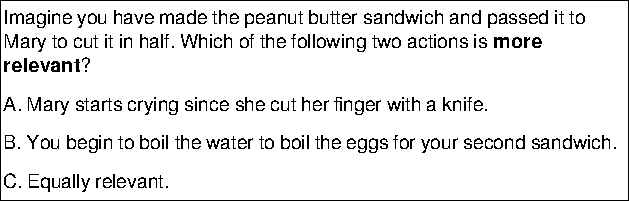
\includegraphics[width=0.48\textwidth]{figure/question-sample4-croped.pdf}
  \vspace*{-7mm}
  \caption{{\fontsize{9}{9}\selectfont Example Relevance Question.}}
  \label{fig:qs1}
  \vspace{-4mm}
\end{figure}

Figure \ref{fig:qs1} shows an example question from the relevance questionnaire
designed to test whether human subjects perceive saliency as a factor in
relevance. In this example, with respect to Algorithm \ref{alg:relevance},
option A is more relevant because of Mary's perceived negative emotion. Although
option B is relevant (since it achieves the next goal in the shared plan), 83\% of
subjects consider it as less relevant than option A; we believe this is due to
the effect of Mary's perceived negative emotion. Option C was provided to
check whether the subjects perceived the other two options as equal. Another
question also tested saliency. However, the options provided only related to the
shared plan (i.e., no human emotions in the options). In this case 87\% of
subjects chose the option that accomplished the next goal in the shared plan.
Interestingly, when confronted with a negative emotion from their collaborator,
human subjects deviated from the shared plan and found their collaborator's
emotion more relevant than the original plan. It is noteworthy that in both the
absence and the presence of emotions the human subjects chose the more salient
option with respect to our definition of saliency, which was not referenced or
provided in the questionnaire. Average results for both questionnaires are
presented in Table \ref{tbl:statistics}.

% \begin{figure}[tbh]
%   \vspace{-1mm}
%   \centering
%   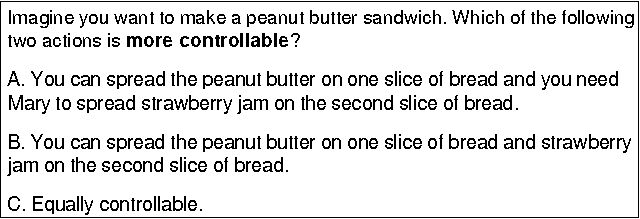
\includegraphics[width=0.48\textwidth]{figure/question-sample2-croped.pdf}
%   \vspace*{-7mm}
%   \caption{{\fontsize{9}{9}\selectfont Example Controllability Question.}}
%   \label{fig:qs2}
%   \vspace{-2mm}
% \end{figure}
% 
% Figure \ref{fig:qs2} shows an example question from the controllability
% questionnaire. The algorithm's output is option B, and is determined by
% Algorithm \ref{alg:controllability} (line 3), similarly to the expectedness
% example above. In this example, option B is more controllable than option A,
% because the self over total ratio of the responsibility of the predecessors of
% the given task (see \textit{Autonomy} in Section \ref{sec:controllability}) is
% higher than the ratio in option A; i.e., self is responsible to spread peanut
% butter on one slice of bread and strawberry jam on another slice of bread. In
% this question, the humans decision was 90\% in agreement with the algorithm's
% output.

% \begin{figure}[tbh]
%   \vspace{-1mm}
%   \centering
%   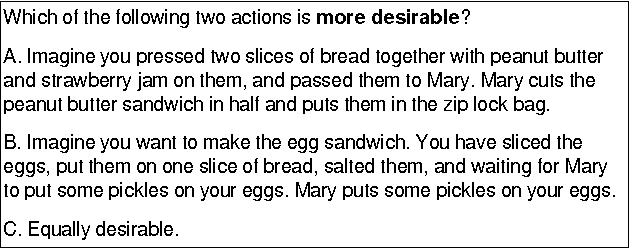
\includegraphics[width=0.48\textwidth]{figure/question-sample3-croped.pdf}
%   \vspace*{-7mm}
%   \caption{{\fontsize{9}{9}\selectfont Example Desirability Question.}}
%   \label{fig:qs3}
%   \vspace{-2mm}
% \end{figure}
% 
% Figure \ref{fig:qs3} shows an example question from the desirability
% questionnaire. The output based on the Algorithm \ref{alg:desirability}
% (line 14) is option C, since in both option A and option B, the focus goal
% has been achieved successfully. Therefore, in this example, both options A and B
% are desirable. The humans decision was 77\% in agreement with the algorithm's
% output in this question.

Our hypothesis in our evaluation was that humans perceive the critical
components used in our algorithms. Each question had 3 answers. Therefore, a
random distribution would result in 33\% agreement with our algorithms'
components. However, the total number of subjects' answers supporting a) the
\textit{relevance} components (n=29) averaged 71.3\% (s=10.7\%), b) the
\textit{controllability} components (n=33) averaged 74.3\% (s=15.8\%). Our
results indicate that people largely performed as our hypothesis predicted. The
\textit{p}-values obtained based on a one-tailed z-test (see Table
\ref{tbl:statistics}) show the probability of human subjects' data being
generated from a random set. The very small \textit{p}-values indicate that the
data set is not random; in fact, the high percentage of similarity shows that
the algorithms' components can help us to model appraisal in a collaboration.

\vspace{-2mm}
\section{Conclusion}
\vspace{-1mm}
As shown in this paper, there are factors involved in appraisal processes
that are not accounted for in existing appraisal models. These factors including
the influence of the human collaborator's emotions must be addressed to provide
proper collaborative behavior in a robot. The SharedPlans theory and other
computational collaboration theories (e.g., Joint Intentions) argue the
importance of commitment in collaboration. According to these theories
collaborators are required to commit to their shared plan or intentions to
successfully collaborate and achieve a shared goal. We believe collaborators'
commitment builds trust. This trust requires them to appraise their environment
based on the shared plan structure, as well as other information that is induced
by the collaboration process, such as the recurrence of a belief by the other
collaborator and the human collaborator's perceived emotion. In our next step,
we want to test our appraisal algorithms and their reciprocal influence on goal
management during collaboration. This study will be conducted between a KUKA
youbot and a human subject on different task model.

% We believe the difference between these two results could be due to several
% reasons, including: a) the fact that we conducted our study online and had
% little control on our subjects, b) our algorithms may require further
% granularity, or c) the difference between decision making processes of
% individuals, which can be affected by other factors such as personality, gender,
% and culture. While it may be possible to achieve a higher level of agreement
% between humans and the algorithms results, these results indicate that the
% current algorithms are adequate to be used in a collaboration context. In our
% future work, we will implement the remaining mechanisms in Affective
% Motivational Collaboration framework and carry out an end-to-end user study to
% verify the behavior of a collaborative robot using our architecture.


% \vspace*{-3mm}
% \section*{Acknowledgments}
% \vspace{-2mm}
% Acknowledgment is suppressed for anonymity.
% \vspace{-4mm}


% {\fontsize{8.2}{9}\selectfont This work is supported by the National Science
% Foundation under award IIS-1012083.}
% Any opinions, findings, and conclusions
% expressed in this material are those of the authors and do not necessarily
% reflect the views of the National Science Foundation.

%% The file named.bst is a bibliography style file for BibTeX 0.99c
\bibliographystyle{named}
\bibliography{mshayganfar}

\end{document}

